\documentclass[a4paper,man,12pt]{article}

% Line spacing
\usepackage{setspace}

\usepackage[margin=1in]{geometry} % Adjust margins if needed

% Section formatting
\usepackage{titlesec}

% Dummy text, remove if not needed
\usepackage{lipsum}

% Graphics and figures
\usepackage{graphicx}
\graphicspath{ {images/} }
\usepackage[rightcaption]{sidecap}
\usepackage{subfig}
\usepackage{wrapfig}

% PDF includes
\usepackage{pdfpages}

% APA 7th edition style citations
\usepackage[style=apa,backend=biber]{biblatex}
\addbibresource{references.bib} % Your bib file

% Title formatting
\usepackage{titlesec}
\titleformat{\section}{\bfseries\large}{\thesection}{1em}{}
\titleformat{\subsection}{\bfseries}{\thesubsection}{1em}{}
\titleformat{\subsubsection}{\itshape}{\thesubsubsection}{1em}{}


% Begin the document
\begin{document}

% --------------- Title Page Section ---------------
% This section is for generating the title page of the research proposal.
% We are using the 'titlepage' environment for this.

\begin{titlepage}
    \begin{center} % All elements will be centered horizontally on the title page
        
        % Insert vertical space to move the title block downwards
        \vspace*{2cm}
        
        % Displaying the document title in large, bold font
        \textbf{\LARGE Research Proposal}
        
        % Insert more vertical space for aesthetic purposes
        \vspace{1.5cm}
        
        % Displaying the specific title of the research in large font
        \textbf{\Large Title of Your Research}
        
        % Additional vertical space for better layout
        \vspace{2cm}
        
        % Displaying the student's ID and name
        \textbf{Student ID, Your Name}
        
        % Fill in remaining vertical space until the next text element
        \vfill
        
        % Displaying the academic programme that the student is enrolled in
        \textbf{Your Programme}
        
        % Another vertical fill to distribute space until the next element
        \vfill
        
        % Displaying the institution details: School, University, and Country
        \textbf{School of Information Technology}\\
        \textbf{Whitecliffe}\\
        \textbf{New Zealand}
        
        % Insert a bit of vertical space for layout
        \vspace{1cm}
        
        % Displaying the current date using LaTeX's \today command
        \textbf{\today}
        
    \end{center} % End centering of elements on the title page
\end{titlepage} % End of title page environment

% --------------- End of Title Page Section ---------------


\pagenumbering{roman}

% The following LaTeX code is for generating an Abstract page in your document.

% Create a new page
\newpage

% Center the content on the page
\begin{center}
    % Add vertical space of 2cm from the top of the page
    \vspace*{2cm}
    
    % Display the title "Abstract" in bold and large font
    \textbf{\Large Abstract}
\end{center}

% Following the title, you should add the content of your abstract.
% You can replace the \lipsum[1] command with your actual abstract content.

% \lipsum[1] is a placeholder text; remove it when adding your own abstract
\lipsum[1] % Remove this and add your own text

% This section of the LaTeX code is for generating the Table of Contents,
% List of Figures, and List of Tables.

% Create a new page for the Table of Contents
\newpage
% Generate the Table of Contents
\tableofcontents
% Create another new page after the Table of Contents
\newpage

% Generate the List of Figures
\listoffigures
% Add the List of Figures to the Table of Contents
\addcontentsline{toc}{section}{List of Figures}
% Create a new page after the List of Figures
\newpage

% Generate the List of Tables
\listoftables
% Add the List of Tables to the Table of Contents
\addcontentsline{toc}{section}{List of Tables}
% Create a new page after the List of Tables
\newpage

% The main content will start here

% Set the page numbering style to Arabic numerals for the main content
\pagenumbering{arabic}
% Reset the page counter to start from 1
\setcounter{page}{1} % Reset page counter to 1


% This section starts the "Introduction" part of the document.
% Use \section to denote a major section in your document.

% Introduction Section
\section{Introduction}

  % The following text introduces the reader to the topic under study.
  % It discusses the problems related to cybersecurity and also refers to a citation.
  
  With the rapid advancement of technology, the IT industry has witnessed a significant increase in cyber threats and attacks. These attacks pose a serious risk to organizations, leading to financial losses, reputational damage, and compromised data. Despite the implementation of various cybersecurity measures, traditional approaches often fall short in detecting and responding to sophisticated and evolving cyber threats \parencite{001}. Therefore, there is a pressing need to explore innovative solutions that can bolster cybersecurity defenses and adapt to emerging threats. This research proposal aims to address this need by investigating the potential of AI in enhancing cybersecurity practices within the IT domain.

  % The \begin{figure} ... \end{figure} environment is used to insert a figure into the document.
  % [!htbp] controls the placement of the figure.
  
  % Insert a figure
  \begin{figure}[!htbp] 
    % Center the figure
    \centering
    % Include an image with a specific width
    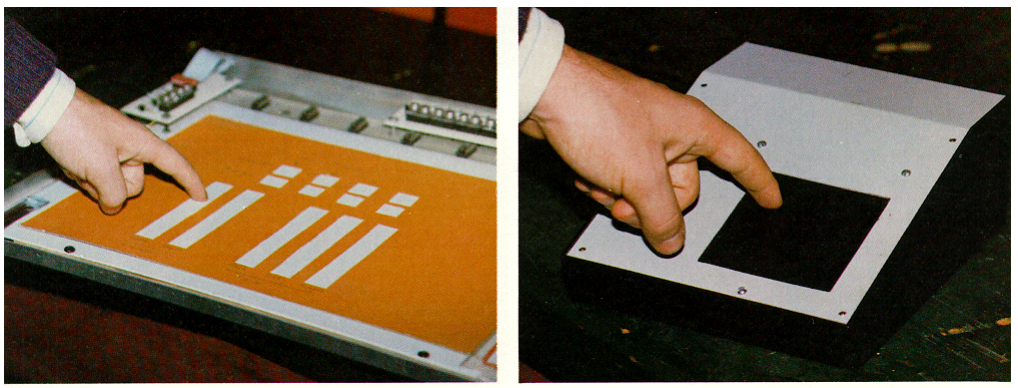
\includegraphics[width=0.75\textwidth]{images/buxton.PNG}
    % Caption for the figure
    \caption{Physical templates proposed by Buxton \parencite{010}}
    % Label to refer to the figure later
    \label{fig:buxton}
  \end{figure}

  % Subsection within the Introduction: Problem Statement
  
  % Use \subsection to denote a subsection within a major section.
  \subsection{Problem Statement}
    
  The feedback received from the first assignment has provided valuable insights into refining the structure and focus of the research proposal. The introduction section has been revised to clearly state the problem statement and highlight the significance of the research. Additionally, the research objectives have been redefined to ensure they align with the research questions and contribute to the overall goal of investigating the impact of AI in cybersecurity \parencite{003,004}. The following sections will delve into the literature review, theoretical framework, research methodology, and other key aspects of the proposed study \cite{012} \textcite{011}.



% The "Literature Review" section starts here.
% Use \section to create a new major section in the document.
\section{Literature Review}

  % The following text provides an overview of what the literature review will cover.
  % It also mentions the types of sources that will be examined and refers to a citation.
  
  The literature review will explore the existing body of knowledge on cybersecurity, AI, and their intersection within the IT domain. It will analyze relevant research papers, articles, and industry reports to identify the current trends, challenges, and advancements in AI-based cybersecurity solutions. The review will encompass topics such as anomaly detection, threat intelligence, intrusion detection systems, and other areas where AI techniques have been successfully applied to enhance cybersecurity practices \paragraph{}
  \cite{001,005,006}.
  
  % Placeholder text (\lipsum) is used here for demonstration purposes.
  % Replace it with the actual text for your literature review.
  
  \lipsum[10] % Remove this to add your text.
  \paragraph{}
  \lipsum[2] % Remove this to add your text.
  \paragraph{}
  \lipsum[2] % Remove this to add your text.
  \paragraph{}
  \lipsum[2] % Remove this to add your text.
  \paragraph{}
  \lipsum[2] % Remove this to add your text.

  % Use \subsection to create a subsection within the "Literature Review".
  % "ABC" is a placeholder title. Replace it with an actual subsection title.
  
  \subsection{ABC}
  \lipsum[2] % Remove this to add your text.
  \paragraph{}
  \lipsum[2] % Remove this to add your text.

  % Another subsection within the "Literature Review".
  % "XYZ" is a placeholder title. Replace it with an actual subsection title.
  
  \subsection{XYZ}
  \lipsum[2] % Remove this to add your text.
  \paragraph{}
  \lipsum[2] % Remove this to add your text.

  % Yet another subsection within the "Literature Review".
  % "ABCXYZ" is a placeholder title. Replace it with an actual subsection title.
  
  \subsection{ABCXYZ}
  \lipsum[2] % Remove this to add your text.
  \paragraph{}
  \lipsum[2] % Remove this to add your text.

  % Use \subsubsection to create a subsubsection within a subsection.
  % "EFG" is a placeholder title. Replace it with an actual subsubsection title.
  
  \subsection{Summary of Literature Review}
  \lipsum[2] % Remove this to add your text.
  \paragraph{}
  \lipsum[2] % Remove this to add your text.




% This section is dedicated to presenting the research questions for the study.
% Use \section to create a new major section in the document.
\section{Research Questions}

  % Placeholder text (\lipsum) is here for demonstration purposes.
  % This should be replaced with an introductory text that sets the context for your research questions.
  
  \lipsum[2] % Remove this to add your text.
  
  % Use \begin{itemize} ... \end{itemize} to create a bulleted list of research questions.
  
  % First set of research questions
  \begin{itemize}
    % Each \item creates a new bullet point in the list.
    
    \item How can AI techniques be utilized to improve the accuracy and effectiveness of cyber threat detection and mitigation?
    \item What are the key challenges and limitations associated with implementing AI-based cybersecurity solutions within the IT industry?
  \end{itemize}

  % Second set of research questions (identical to the first set in this example)
  % If these are supposed to be the same as the previous list, you may want to explain why you're repeating them.
  
  \begin{itemize}
    \item How can AI techniques be utilized to improve the accuracy and effectiveness of cyber threat detection and mitigation?
    \item What are the key challenges and limitations associated with implementing AI-based cybersecurity solutions within the IT industry?
  \end{itemize}


% This section is for presenting the research objectives.
% Use \section to create a new major section in your document.
\section{Research Objectives}

  % Placeholder text (\lipsum) is here for demonstration purposes.
  % It should be replaced with an introductory text that sets the stage for your research objectives.
  
  \lipsum[2] % Remove this to add your text.

  % Use \begin{itemize} ... \end{itemize} to create a bulleted list of research objectives.
  % Each \item starts a new bullet point in the list.
  
  \begin{itemize}
    % The first research objective, focusing on developing an AI-driven framework.
    \item Develop an AI-driven cybersecurity framework that integrates machine learning algorithms for proactive threat detection.

    % The second research objective, focusing on evaluating the performance of the proposed framework.
    \item Evaluate the performance and effectiveness of the proposed framework in comparison to traditional cybersecurity approaches.
  \end{itemize}



% This section is for outlining the theoretical framework of the research.
% Use \section to create a new major section in your document.
\section{Theoretical Framework}

  % This paragraph serves as an introduction to the theoretical framework.
  % It outlines what topics the framework will cover and how it will guide the research.
  % The theoretical framework is critical for understanding the basis of the research, 
  % including the concepts, theories, and methodologies that will be used.

The theoretical framework will provide the conceptual basis for the research by exploring the underlying principles and concepts related to AI, cybersecurity, and their interplay. It will encompass topics such as supervised and unsupervised machine learning, neural networks, data preprocessing, feature extraction, and model evaluation techniques. The framework will guide the development and implementation of the AI-driven cybersecurity solution proposed in this research.



% This section discusses the Research Methodology.
% Use \section to introduce a new major section in your document.
\section{Research Methodology}

  % The following paragraph is an introduction to the research methodology.
  % It outlines the various steps, procedures, and ethical considerations that will be taken into account during the research.
  % Important aspects like data collection, AI algorithm implementation, and evaluation metrics are mentioned.
  
  The research methodology will outline the steps and procedures to be followed in conducting the study. It will describe the data collection process, including the sources of cybersecurity data and datasets used for training and evaluation. The methodology will also detail the implementation of AI algorithms, the evaluation metrics employed, and the statistical analysis techniques applied to measure the performance of the proposed cybersecurity framework. Ethical considerations, such as data privacy and confidentiality, will be addressed to ensure compliance with ethical standards in research.



% This section is dedicated to the discussion of Ethics in the research.
% The \section command introduces a new major section in the document.
\section{Ethics}

  % The following paragraph outlines the ethical considerations for the research.
  % It discusses the importance of ethics, especially in the realm of cybersecurity research.
  % Topics such as data privacy, anonymity, and algorithmic bias are mentioned.
  
Ethical considerations play a crucial role in conducting research, particularly in the field of cybersecurity. This research will adhere to ethical guidelines by ensuring the privacy and anonymity of individuals and organizations whose data is used for analysis. Data will be obtained from legal and authorized sources, and proper consent will be sought whenever necessary. The research will also consider the potential biases and limitations associated with AI algorithms, striving to mitigate any adverse impacts on individuals or groups.



% This section is for outlining the Expected Results of the research.
% The \section command introduces a new major section in your document.
\section{Expected Results}

  % The paragraph below discusses how the research findings will be communicated.
  % It highlights the various channels through which results will be disseminated, including academic conferences and journals.
  % The objective is to inform a broad audience, ranging from researchers to industry professionals, about the potential of AI in cybersecurity.
  
  The research findings will be disseminated through various channels to ensure effective communication of results. This will include academic conferences, journal publications, and presentations to industry professionals and stakeholders. The communication of results will aim to raise awareness about the potential of AI in improving cybersecurity practices within the IT domain and facilitate knowledge exchange among researchers, practitioners, and organizations in the field.



% This section is for discussing the Significance of the Research.
% The \section command introduces a new major section in your document.
\section{Significance of Research}

  % This paragraph elaborates on why the research is important.
  % It discusses the potential contributions to both the academic field and the IT industry.
  % Topics such as improving cybersecurity measures, reducing false positives, and contributing to further research are highlighted.
  
  The significance of this research lies in its potential to advance the field of cybersecurity within the IT industry. By leveraging AI techniques, organizations can enhance their capabilities to detect, prevent, and respond to cyber threats more efficiently. The proposed AI-driven cybersecurity framework has the potential to significantly reduce false positives and improve the overall accuracy of threat detection, thereby bolstering the resilience of organizations' digital infrastructure. Moreover, the research findings will contribute to the academic and practical understanding of AI in cybersecurity, paving the way for further research and innovation in this domain \cite{015}.


% This section is for Critical Reflection.
% The \section command introduces a new major section in your document.
\section{Critical Reflection}

  % This paragraph introduces the critical reflection task.
  % It asks the reader to consider ethical issues and potential barriers to research.
  % Ngā Tikanga Paihere framework is mentioned as the basis for ethical considerations.
  
  The third task in this assessment asks you to critically reflect on ethical issues and/or potential barriers to undertaking the proposed research. Using Ngā Tikanga Paihere as a framework, explore, analyse and critically reflect on the ways in which these principles will be integrated and mitigate emerging ethical issues and/or potential barriers to your research. It is important to understand the significance of Ngā Tikanga Paihere principles and which ones relate to your research and consider their impact on your research.

% This section is for the Conclusion of the research.
% The \section command introduces a new major section in your document.
\section{Conclusion}

  % Placeholder text (Lorem Ipsum) is used for now.
  % Replace this with your own text to discuss the research's conclusions.
  
  \lipsum[2]
  \paragraph{}
  
  % Another placeholder text.
  % Again, this should be replaced with your own text.
  
  \lipsum[2]




% This section discusses the Budget for the research.
% The \section command introduces a new major section in your LaTeX document.
\section{Budget}

  % The following lines introduce what the budget will cover and estimates its total amount.
  
  The budget for this research proposal will primarily cover the following aspects:
  The total budget for this research project is estimated at \$40,000.

  % The table environment is initiated for displaying budget information.
  % The 'ht' parameter suggests placing the table here or at the top of the page.
  
  \begin{table}[ht]
    \centering % Centers the table horizontally on the page
    
    % The \caption and \label commands provide a title and label for the table, respectively.
    
    \caption{Budget Information}
    \label{tab:budget}
    
    % The tabular environment sets up the structure of the table.
    % In this case, it has three columns: one left-justified and two right-justified.
    
    \begin{tabular}{|l|r|r|}
      \hline % Draws a horizontal line
      
      % The table header is created using \textbf for bold text.
      
      \textbf{Category} & \textbf{Budgeted Amount (\$)} & \textbf{Actual Amount (\$)} \\
      \hline % Another horizontal line
      
      % The table rows, containing the budget categories and their amounts.
      
      Salaries & 5000 & 5200 \\
      Rent & 1200 & 1200 \\
      Supplies & 500 & 480 \\
      Advertising & 800 & 900 \\
      Miscellaneous & 300 & 250 \\
      
      \hline % Another horizontal line
      
      % The table footer, showing the total budgeted and actual amounts.
      
      \textbf{Total} & \textbf{7800} & \textbf{8030} \\
      
      \hline % Final horizontal line
    \end{tabular}
  \end{table}


% This is the References or Bibliography section.
% A new page is started with \newpage.
% The \printbibliography command lists all cited works.

\newpage
\printbibliography

\newpage

% Start the Appendix
\appendix

% Change section title format to be centered
\titleformat{\section}[block]{\normalfont\Large\bfseries\centering}{\thesection}{1em}{}

\section{Timeline} % Create a new section for the Timeline in the Appendix

% Reset section title format to LaTeX default
\titleformat{\section}[block]{\normalfont\Large\bfseries}{\thesection}{1em}{}

% Include the Gantt chart PDF
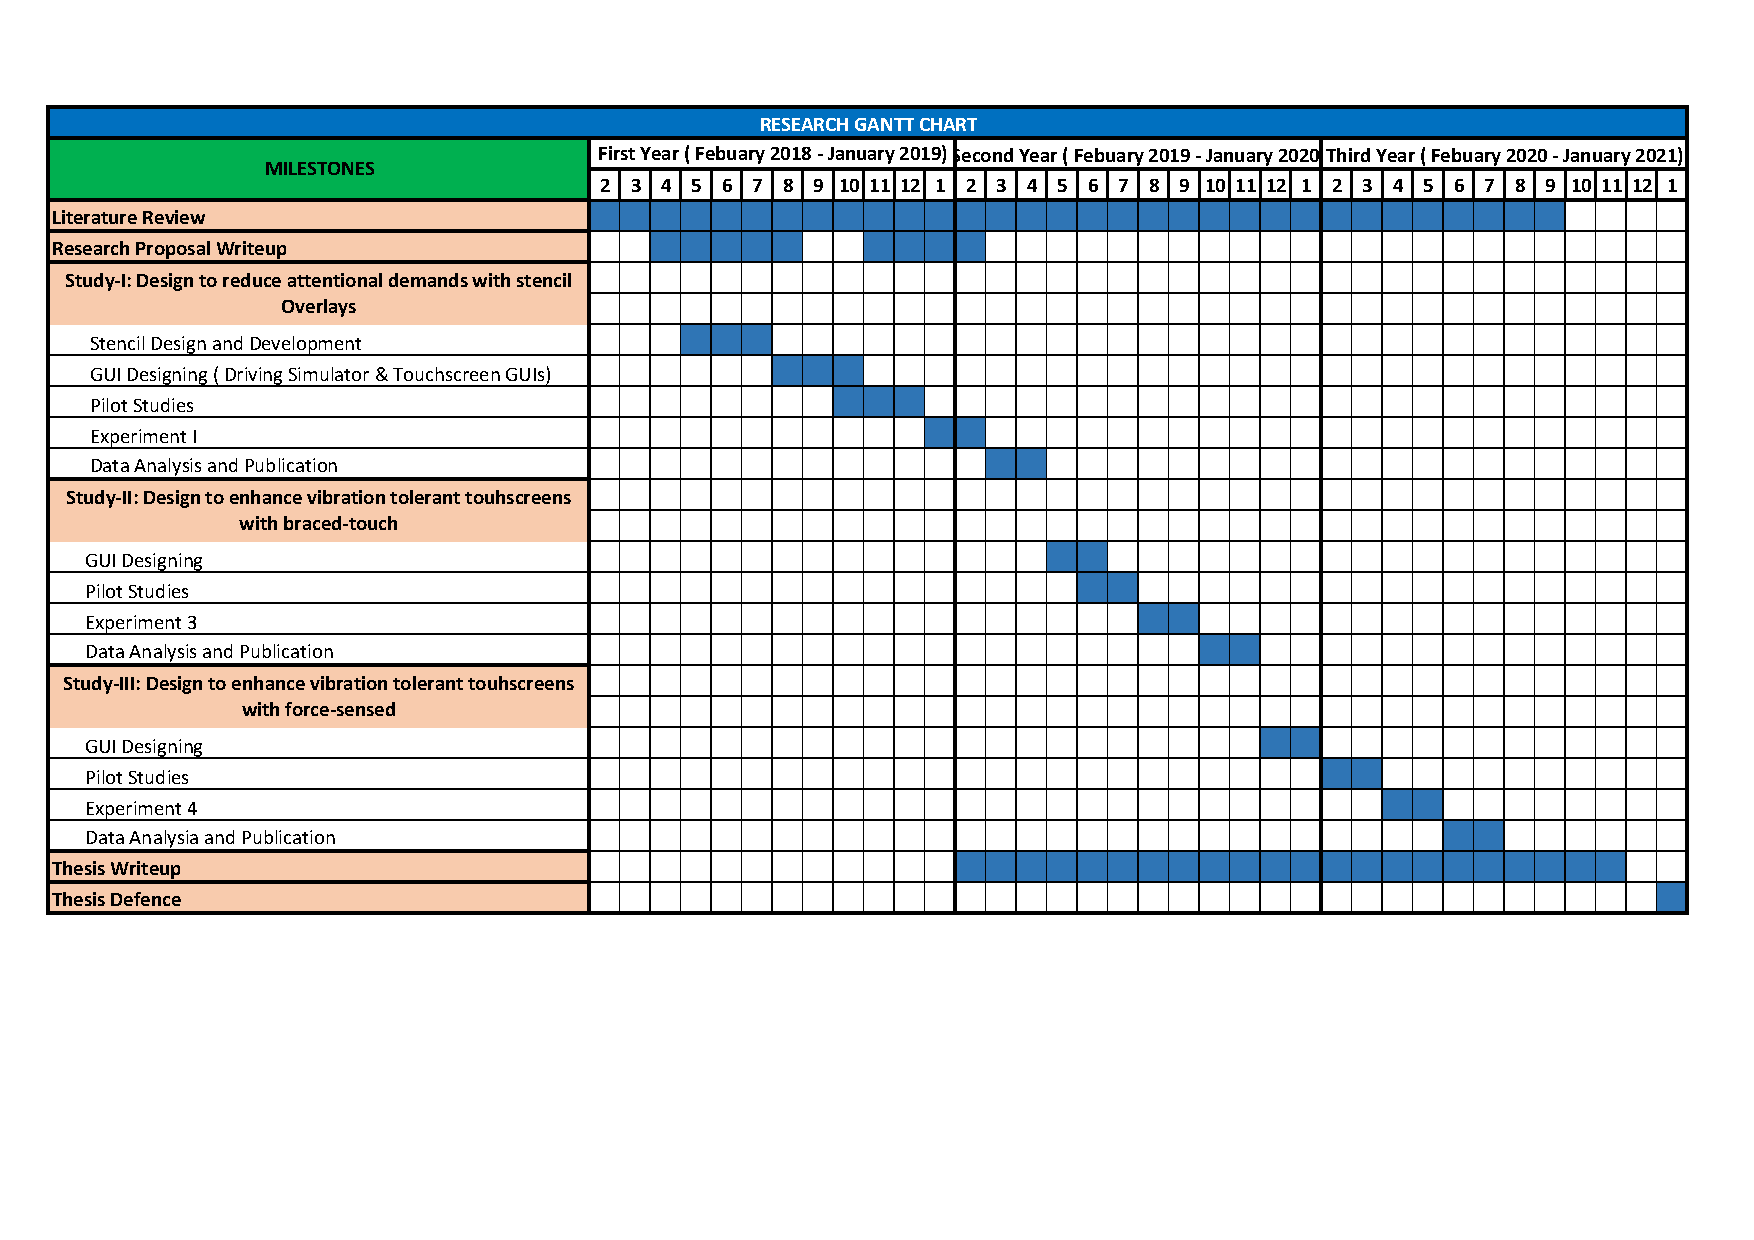
\includepdf[pages={-}, angle=90, scale=0.9]{Gantt-Chart.pdf}

% The \end{document} command indicates the end of the LaTeX document.
\end{document}
